\chapter{Metodologia}
\label{Metodologia}
%\externaldocument[met-]{metodologia}


Neste capítulo são apresentados os conceitos do algoritmo imperialista competitivo e a apresentação da operação de convolução e a convolução de imagens, seguidos de uma breve análise sobre estes assuntos, direcionando como estes conceitos serão aplicados na bisca da solução do problema proposto.

\section{Algoritmo Imperialista Competitivo}

O algoritmo imperialista competitivo \cite{atashpaz2007imperialist} (ou ICA - \emph{Imperialist Competitive Algorithm} em inglês) é um algoritmo evolutivo baseado na ideia da disputa entre impérios pela extensão de seus domínios para além de seus territórios. Para que um império aumente seu poder ele deve aplicar sua influência sob mais territórios dominando-os e assimilando-os. Territórios dominados por países imperialistas são chamados de colônias, e um império é denominado pelo conjunto formado por um país imperialista e suas colônias.

As colônias de um império tendem a ter suas características se assemelhando às de seu país imperialista a cada década que passa. Esta tendência pode ser vista como uma forma de movimento, ou seja, uma colônia se move em direção ao seu país imperialista de forma que suas características se pareçam mais com as dele.

A definição do poder dos países, sejam eles imperialistas ou colônias, é baseado na ideia de que um dado país tem um custo para se manter. Se um país é rico em recursos, significa que ele terá um custo muito baixo, e consequentemente poderá usar seus recursos de forma a expandir suas fronteiras através da assimilação de colônias. Assim o poder de um país é definido pelo inverso de seu custo, implicando em quando um país possuir um custo muito próximo de (ou tender a) zero, isto significará que seu poder seria imenso e tenderia a infinito.

Antes que a disputa imperialista comece, todos os países são gerados com características aleatórias. Os custos dos países gerados são calculados, e consequentemente seus poderes são definidos. Uma porcentagem dos países com maior poder se tornam impérios, e o restante se tornam colônias. As colônias são distribuídas aos impérios mais poderosos de uma forma proporcional.

Impérios disputam entre si usando como forma de medição o nível de poder total, que por sua vez é definido pela soma do poder do país imperialista com o poder de suas colônias. Assim, um países imperialistas mais fortes tendem a tomar as colônias de um imperialista mais fraco, e os imperialistas mais fracos tendem a perder suas colônias para imperialistas mais fortes até que eles não tenham mais nenhuma colônia e sejam eliminados da disputa. 

Uma colônia pode se tornar um país imperialista quando seu poder superar o poder de seu atual imperialista, assim, todas as colônias do país imperialista, incluindo ele mesmo, passam a ser colônias da colônia que se tornou o novo país imperialista, alterando assim, a direção do movimento das colônias para a posição deste novo imperialista.

O resultado deste processo competitivo tende para que reste apenas um império na disputa possuindo todas as colônias, de forma que todas as colônias tenham as mesmas características poder de seu país imperialista.

Sendo o ICA um algoritmo evolutivo, seu objetivo é encontrar uma solução dentre diversas outras, tal que esta seja ótima, em termos das variáveis do problema (dimensões) em questão.  Como pode ser visto na figura Fluxograma ICA antes de começar o processo evolutivo, deve-se inicializar os países formando os impérios e as suas respectivas colônias. Sendo assim, inicialmente deve-se definir a estrutura básica de um país que, analogamente a um cromossomo presente no algoritmo genético canônico (GA - \emph{Genetic Algorithm}), usa um vetor de valores de dimensão \(1xN_{var}\) apresentado pela equação \ref{eq:ica1}:

\begin{equation}
\label{eq:ica1}
\text{país} = [p_{1},p_{2},...,p_{N_{var}}] 
\end{equation}

Sendo que os elementos contidos no vetor representem as características deste país com valores numéricos de ponto flutuante, diferentemente do GA canônico, que usa uma tripa de valores booleanos que geralmente devem ser traduzidos quando se deseja usar valores numéricos. E define-se \(N_{var}\) o número de dimensões do problema a ser otimizado. 

\begin{figure}[h]
	\centering	
	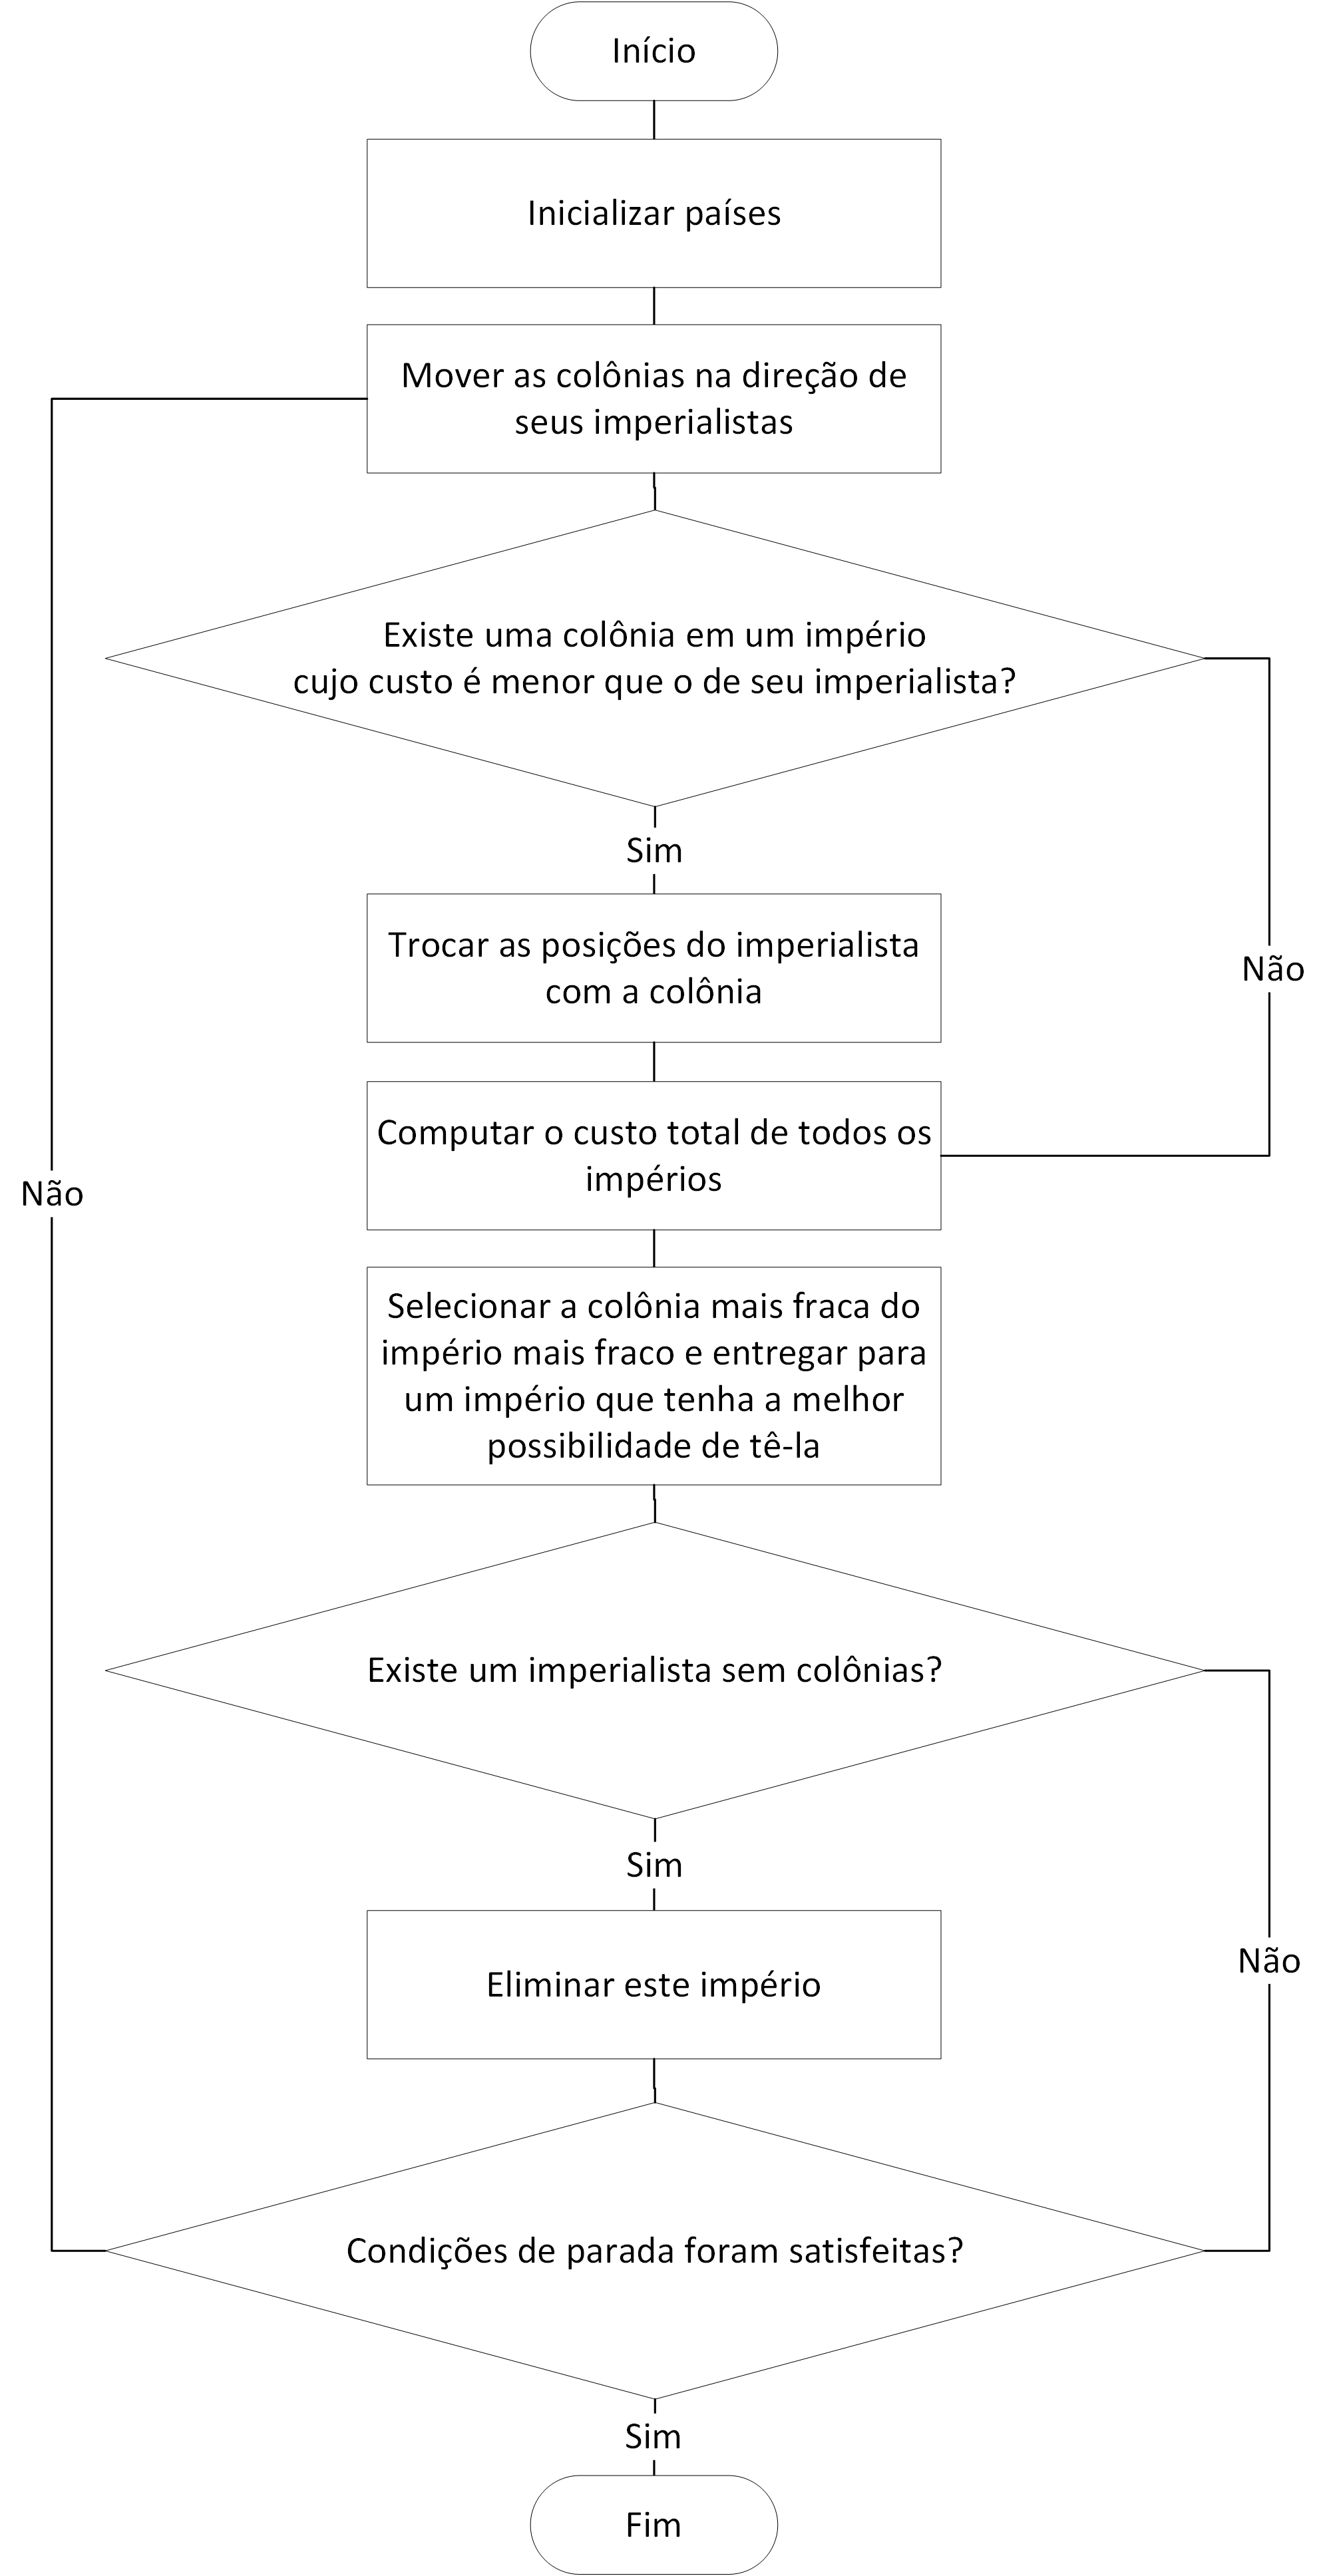
\includegraphics[scale=0.55]{Figuras/Fluxograms-ICACanonic.png}
	\caption{Fluxograma ICA canônico}
	\label{fig:Fluxograms-ICACanonic}
	\end{figure}

O custo de um país deve ser calculado através da aplicação dos valores presentes no país a uma função \(f\) de acordo com a equação \ref{eq:ica2}:

\begin{equation}
\label{eq:ica2}
custo = f (\text{país}) = f (p_{1},p_{2},...p_{N_{var}})
\end{equation}

Sendo o custo um valor análogo ao valor de aptidão de um cromossomo no algoritmo genético e \(f\) uma função de avaliação.

Um valor inicial \(N_{pop}\) define a quantidade de países que serão gerados com valores (características) aleatórios na sua inicialização, antes que se comece a etapa de otimização (competição imperialista). Seleciona-se também uma porção de \(N_{pop}\), denominada \(N_{imp}\), como sendo o número de países imperialistas inicial. A partir disso, são escolhidos como os \(N_{imp}\) países imperialistas, os países mais poderosos dentre os \(N_{pop}\) países. A quantidade de países restantes é denominada \(N_{col}\), tal como mostra a equação \ref{eq:ica3}: 

\begin{equation}
\label{eq:ica3}
N_{col} = N_{pop} - N_{imp} 
\end{equation}

E que posteriormente serão distribuídas proporcionalmente a cada um dos imperialistas.

Para a distribuição  das \(N_{col}\) colônias para os \(N_{imp} \) imperialistas ser feita de modo proporcional ao poder de cada um destes países imperialistas, define-se o valor normalizado do custo de um imperialista segundo a equação \ref{eq:ica4}

\begin{equation}
\label{eq:ica4}
C_{n} =  c_{n} - maxi{c_{i}}
\end{equation}

Onde \(C_{n}\) é o custo normalizado do n-ésimo imperialista, \(c_{n}\) é o custo normalizado deste enésimo imperialista, e a operação \(maxi{c_{i}}\) representa o valor máximo dos custos dentre todos os países. Assim, pode-se definir o poder normalizado de cada país imperialista como mostra a equação \ref{eq:ica5}:

\begin{equation}
\label{eq:ica5}
P_{n} = \left| \frac{C_{n}}{\sum_{i=1}^{Nim}C_{i}}\right| 
\end{equation}

Que é basicamente o custo normalizado do enésimo imperialista dividido pela soma dos custos normalizados dentre todos os imperialistas. Sendo assim, este poder normalizado pode ser entendido como um valor que representa a porção de colônias que devem ser possuídas por aquele imperialista. Então o número de colônias de um império é definido pela equação \ref{eq:ica6}:

\begin{equation}
\label{eq:ica6}
N.C.n = arredondamento ( P_{n} \cdot N_{col})
\end{equation}

Sendo \(N.C.n\) o número inicial de colônias do enésimo imperialista.

Com os impérios já formados, contendo um país imperialista e suas colônias, a sequencia do fluxograma indica que as colônias de um império devem se movimentar em direção ao seu país imperialista, como pode ser visto na Figura\ref{fig:Ilustrations-ColonyEmpireMove}. O movimento de uma colônia até seu imperialista deve ser calculado considerando um fator aleatório e um fator de controle de intensidade, sendo que o fator aleatório pode ser de distribuição uniforme (ou qualquer outra que seja apropriada a situação) e  o fator de controle de intensidade deve ser relativo ao império, portanto usa-se a distância entre o imperialista e a colônia. Assim, tem-se que um valor \(x\), representado o movimento que será efetuado pela colônia, seja o produto vetorial entre a distância e o fator aleatório, como mostrado na equação \ref{eq:ica7} a seguir:

\begin{equation}
\label{eq:ica7}
x  = URand(0, \beta \times d)
\end{equation}

Sendo \(\beta\) um valor aleatório maior que 1 e \(d\) a distância absoluta entre o país imperialista e a colônia.

\begin{figure}[h]
	\centering	
	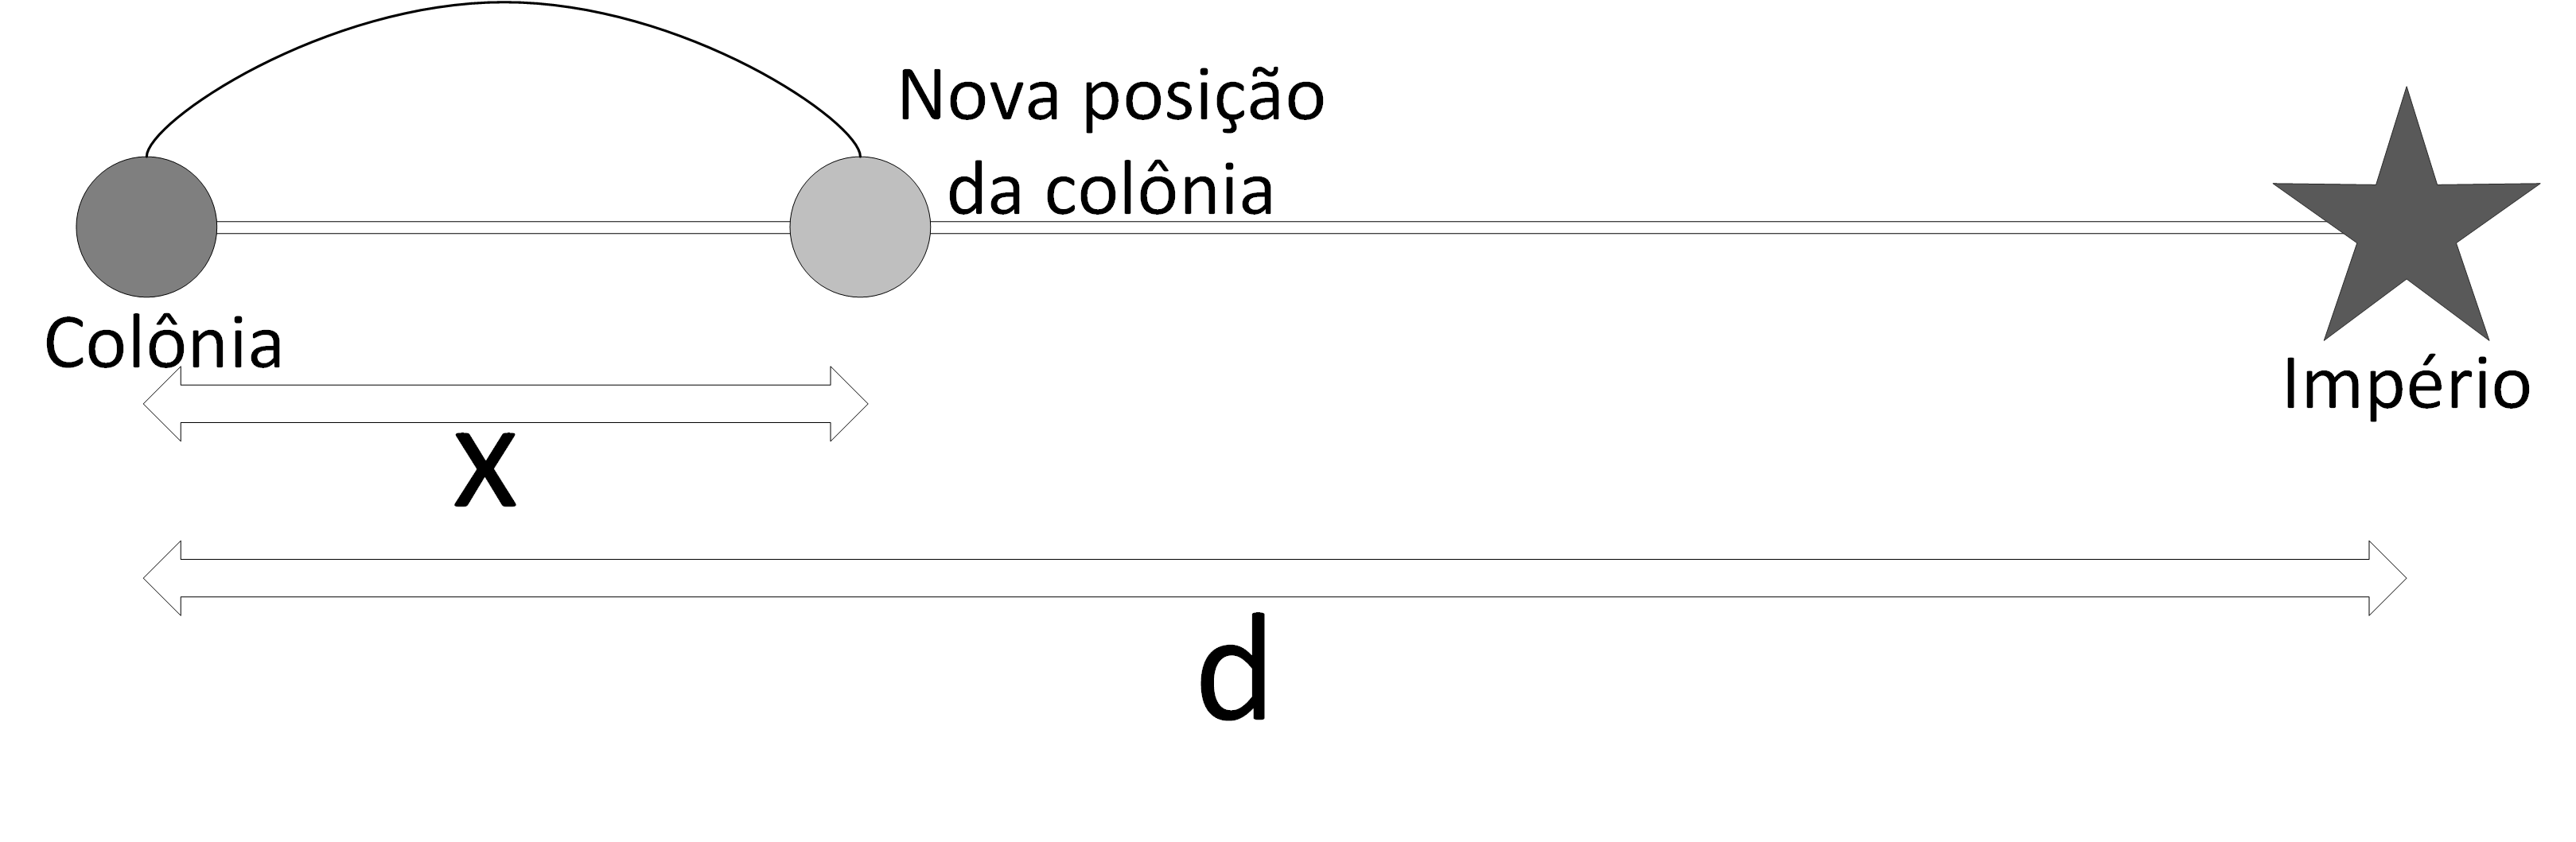
\includegraphics[scale=0.5]{Figuras/Ilustrations-ColonyEmpireMove.png}
	\caption{Movimento da colônia para seu imperialista}
	\label{fig:Ilustrations-ColonyEmpireMove}
\end{figure}

Usa-se \(\beta\) maior que 1 por resultar em um efeito elástico no espaço de busca, fazendo que uma colônia se aproxime de seu imperialista explorando ambos os lados como pode ser visto na Figura \ref{fig:Ilustrations-BetaComparison}. 

\begin{figure}[h]
	\centering	
	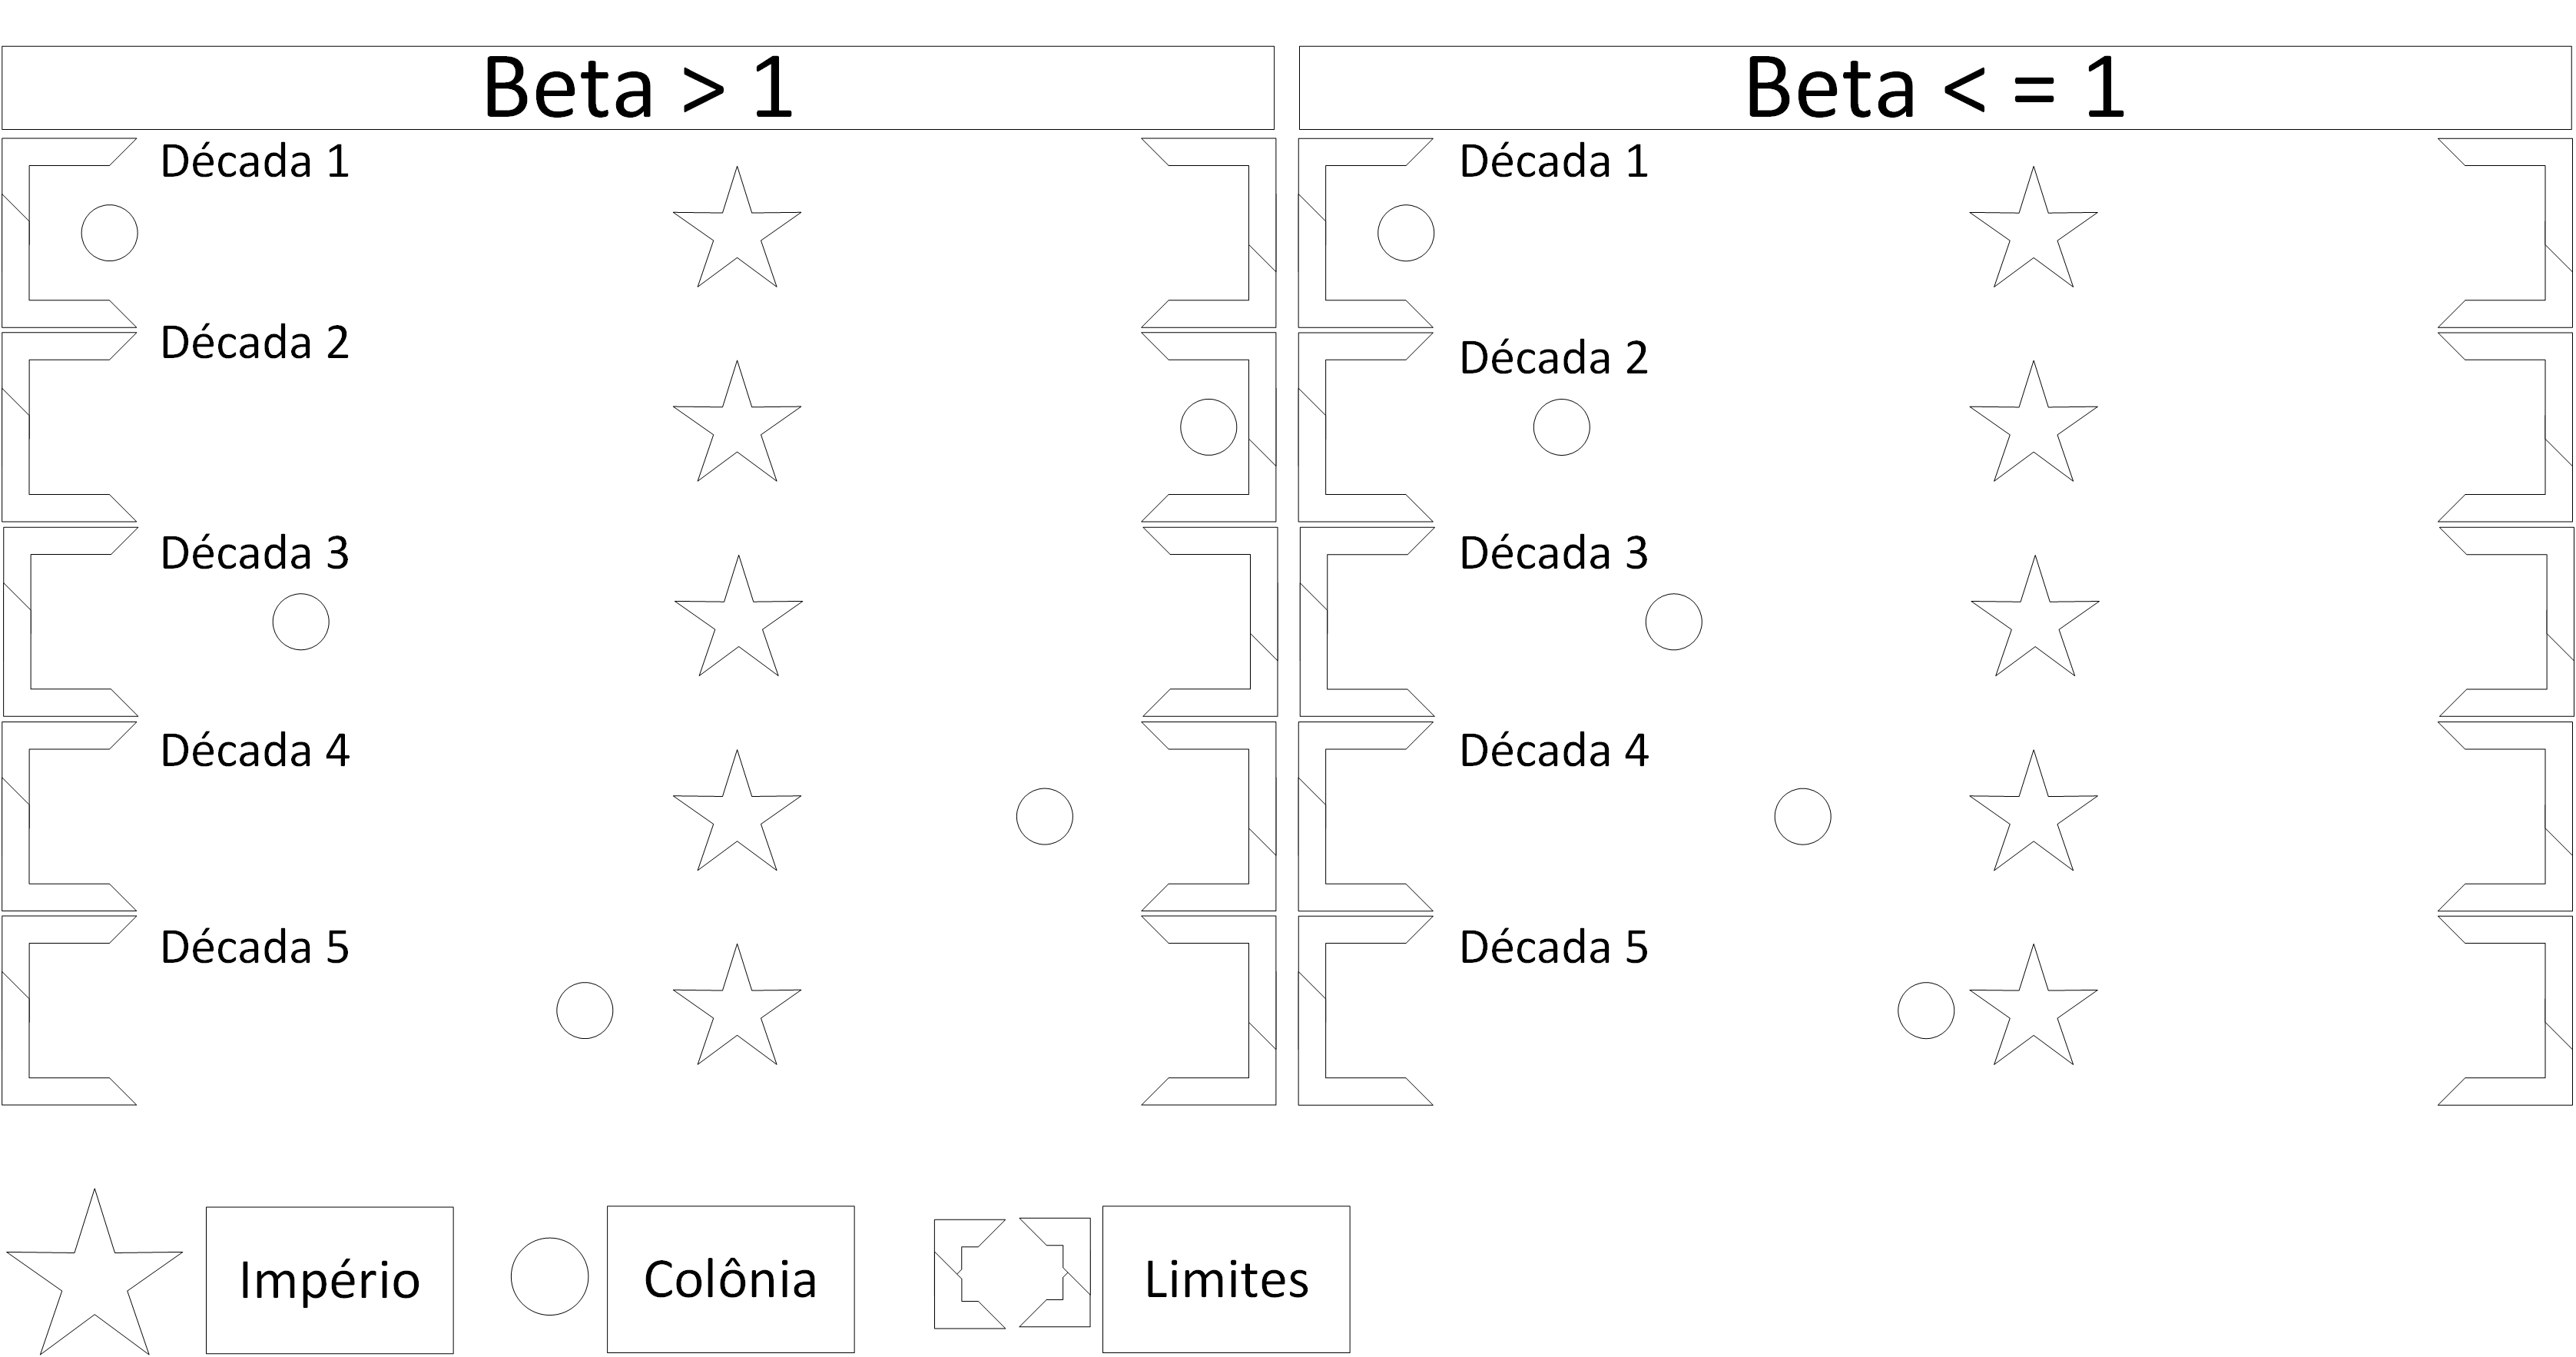
\includegraphics[scale=0.5]{Figuras/Ilustrations-BetaComparison.png}
	\caption{Comparação $\beta$ \textless 1 e $\beta$ \textgreater 1}
	\label{fig:Ilustrations-BetaComparison}
\end{figure}

Para que se tenha uma busca mais diferenciada, e que explore pontos mais diferenciados ao redor do país imperialista, ainda há a adição de um valor aleatório de desvio na direção do movimento , como mostrado na Figura \ref{fig:Ilustrations-ColonyEmpireMoveWithDistortion}. \(\theta\) é um outro valor aleatório de distribuição uniforme(ou qualquer outra que seja apropriada a situação), tal que seus limites sejam inversos e de mesma intensidade Gama, como:

\begin{equation}
\label{eq:ica8}
\theta = URand(-\gamma, \gamma)
\end{equation}

Onde \(\gamma\) é o parâmetro de ajuste de desvio da direção original. Sendo assim, a nova posição da colônia pode ser entendida como um ponto aleatório proporcional a distância entre esta colônia e seu imperialista, que explora as redondezas do imperialista limitando-se na distância e com a adição de um ruído para a exploração mais dinâmica do espaço de busca.

\begin{equation}
\label{eq:ica9}
\text{Posição} (t+1) = \text{Posição}(t) + x + \theta
\end{equation}

\begin{figure}[h]
	\centering	
	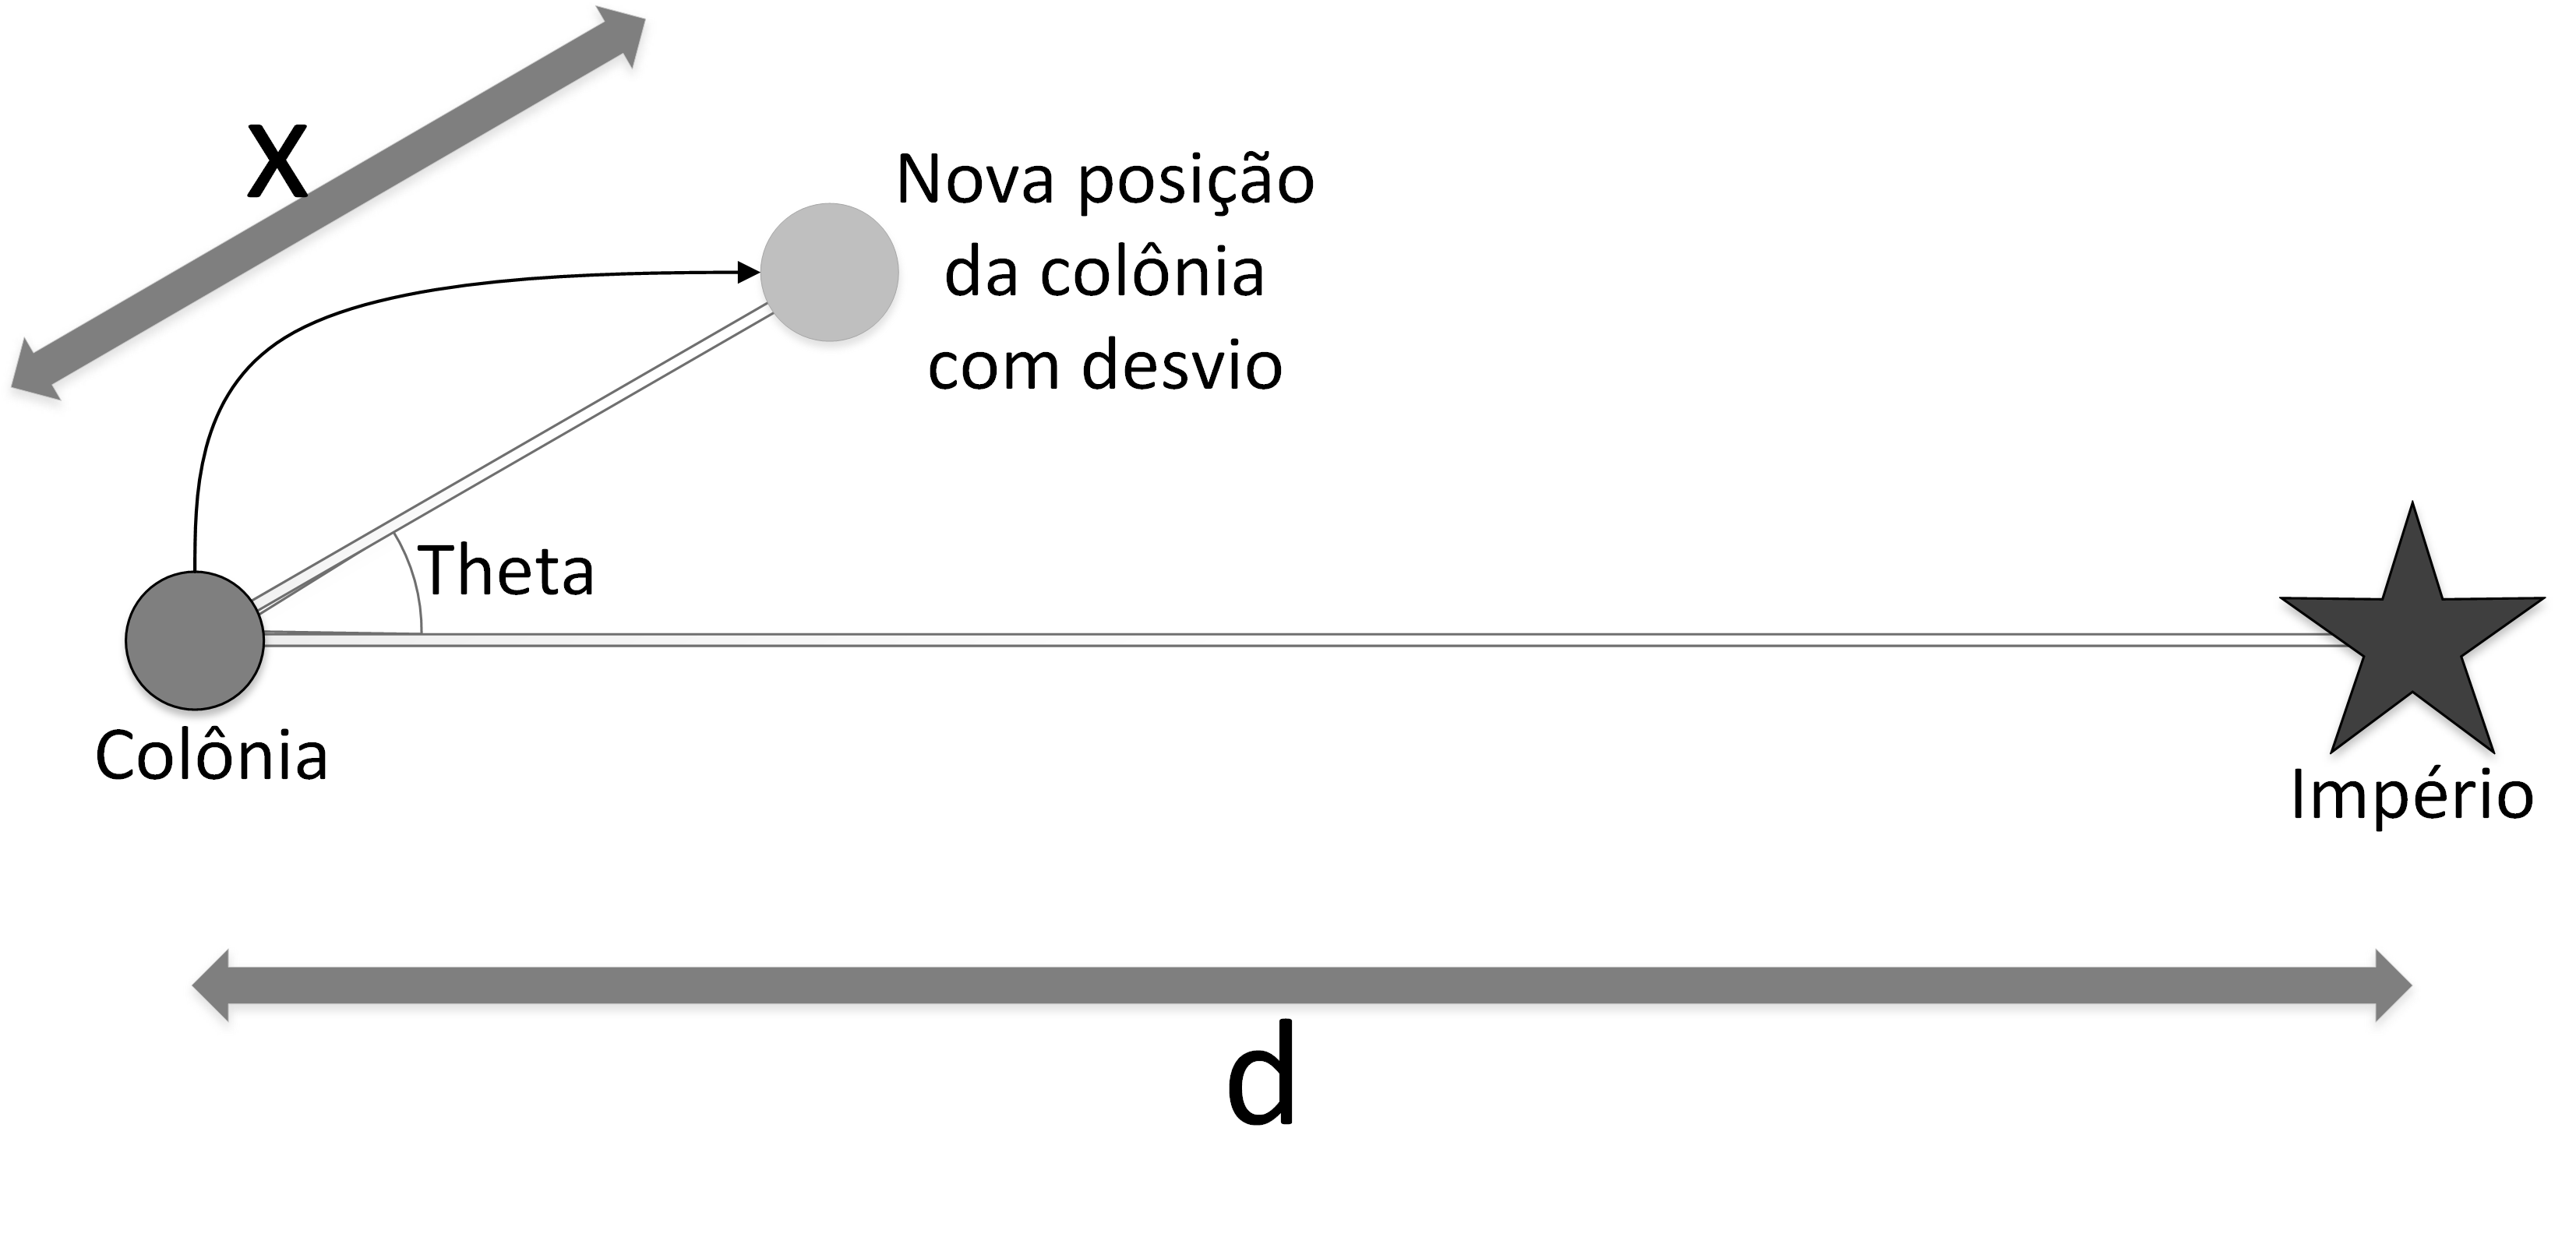
\includegraphics[scale=0.5]{Figuras/Ilustrations-ColonyEmpireMoveWithDistortion.png}
	\caption{Movimento da colônia para seu imperialista com desvio de direção}
	\label{fig:Ilustrations-ColonyEmpireMoveWithDistortion}
\end{figure}

Este processo de movimentação é executado para todas as colônias de cada país imperialista, assim que todas as colônias terminam sua movimentação, ainda é possível haver o que é chamado de processo de revolução, ou apenas revolução, que é uma operação muito semelhante a operação de mutação no GA, onde todas as características (valores do vetor país) da colônia são geradas novamente de forma aleatória.

A segunda etapa, seguindo o fluxograma, faz a verificação dentre todos os imperialistas se uma de suas colônias possui características melhores que seu país imperialista, assim a colônia passa a ser o país imperialista tomando todas as colônias deste antigo imperialista em questão e inclusive, tornando este país imperialista uma colônia. Situações como esta ocorrem quando a colônia ao mover em direção ao seu país imperialista acaba se posicionando em um local onde suas características passam a apresentar um custo menor que o custo de seu país imperialista, como pode ser visto na Figura\ref{fig:Ilustrations-ColonialRevolution}. Nesta mesma figura, observa-se o movimento de colônias em direção ao sei país imperialista (quadro 1), e quando uma colônia passa por uma posição melhor que a de seu país imperialista (quadro 2), ela altera a sua cor e inicia o processo de tomada do império para si, se tornando o novo império, assimilando as colônias do antigo império e consequentemente transformando este antigo imperialista em uma colônia (quadro 3). Posteriormente, observa-se que as colônias passam a se movimentar em direção a este novo imperialista (quadro 4).

\begin{figure}[h]
	\centering	
	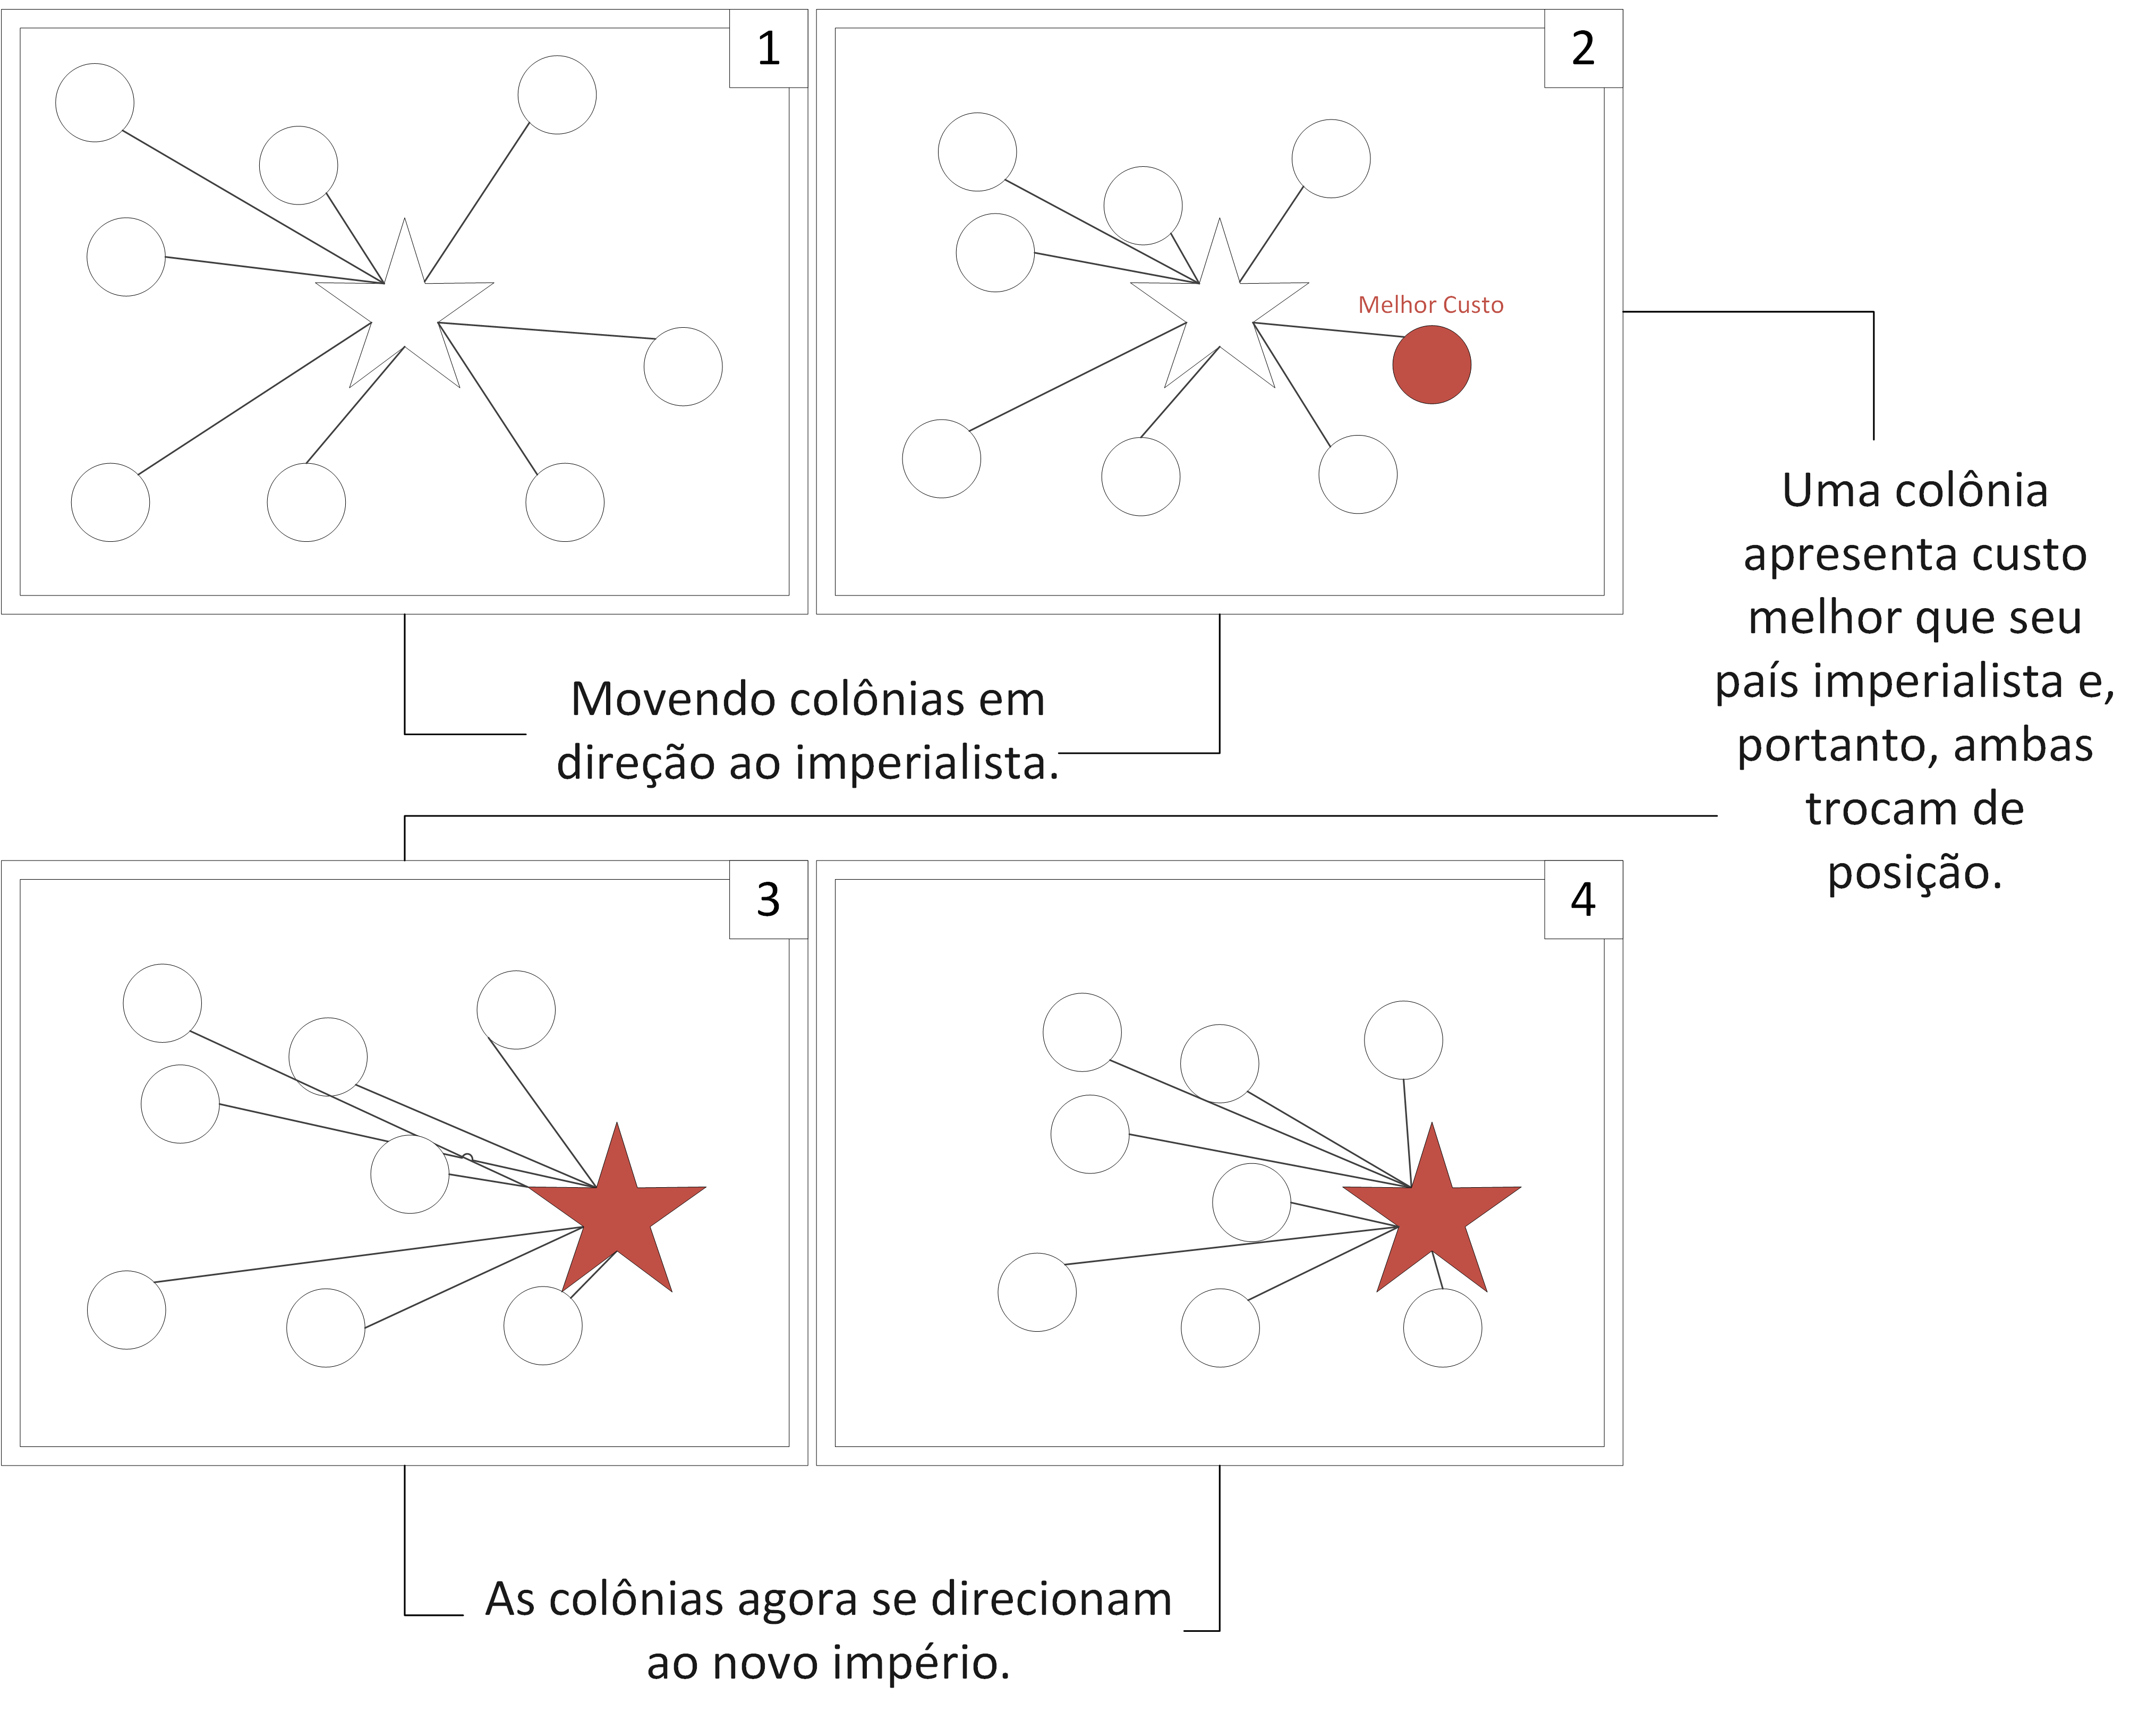
\includegraphics[scale=0.5]{Figuras/Ilustrations-ColonialRevolution.png}
	\caption{Tomada de império por colonia}
	\label{fig:Ilustrations-ColonialRevolution}
\end{figure}

Em seguida, o próximo passo, após as trocas entre impérios e colônias(caso existam), é o cálculo de todos os custos totais dos impérios, que também leva em consideração o valor do custo de suas colônias. Assim, define-se custo total de um império, como sendo a soma entre o custo do país imperialista mais uma porção da média dos custos das colônias pertencentes a este império, definido pela equação \ref{eq:ica10}:

\begin{equation}
\label{eq:ica10}
T.C.n =   Custo(Imperialista n) + \\
 \epsilon \cdot \text{Média}(Custo(Colonias do \text{império} n))
\end{equation}

No qual T.C.n é o custo total do enésimo imperialista, \(\epsilon\)  é o valor que define o quanto a média dos custos das colônias do enésimo império influenciará no custo total, sendo \(\epsilon\) menor que 1. O cálculo do custo total de um império é usado para calcular o poder de um império durante a competição imperialista. Assim, quando usa-se um valor muito baixo para \(\epsilon\) o poder do império será definido basicamente pelo custo do país imperialista, e quando aumenta-se este valor, os custos das colônias passam ter uma maior influência no poder do império, o qual implica diretamente na competição imperialista, ou seja, se o império tem um custo baixo, porém as suas colônias tem custos muito altos, se \(\epsilon\) for baixo, este império tem maiores chances de ganhar uma competição imperialista do que se este valor de \(\epsilon\) fosse um valor mais alto.

A partir deste ponto inicia-se a competição imperialista, que se resume em selecionar a colônia mais fraca do império mais fraco e colocá-la sob o comando de um império que tenha a maior afinidade para tê-la. Assim, a competição imperialista é uma forma de aumentar o poder dos melhores impérios e diminuir o poder dos piores impérios. O império com mais chances de tomar uma colônia para si é aquele com maior poder dentre os impérios competidores, porém não é sempre que o império mais poderoso adquire a colônia em jogo, lembrando que quem adquire a colônia é aquele que tem maior afinidade para tê-la, e não maior poder. Assim, para definir o país com maior afinidade de possessão durante a competição imperialista, usa-se os valores de custo total dos impérios, calculados no passo anterior, para calcular o custo total normalizado, como mostra a equação \ref{eq:ica11}:

\begin{equation} 
\label{eq:ica11}
N.T.C.n = T.C.n - max(T.C.i)
\end{equation}

Sendo \(N.T.C.n\) o valor normalizado do custo total do enésimo império, \(T.C.n\) o custo total do enésimo império e \(max(T.C.i)\) o máximo valor dentre todos os custos totais. Assim que se calculam todos os custos normalizados, calcula-se as probabilidades de possessão de cada imperialista como mostra a equação \ref{eq:ica12}:

\begin{equation} 
\label{eq:ica12}
P_{pn} = \left| \frac{N.T.C.n}{\sum_{i=1}^{N_{imp}}N.T.C.i} \right| 
\end{equation}

Com estes valores de probabilidades de possessão para cada império, cria-se o vetor \(P\), apresentado pela equação \ref{eq:ica13}:

\begin{equation} 
\label{eq:ica13}
P = [P_{p1}, P_{p2}, ..., P_{pN_{imp}}] 
\end{equation}

Cria-se também o vetor \(R\), com o mesmo tamanho de \(P\) porém preenchido com valores aleatórios distribuídos uniformemente e limitados entre 0 e 1, tal como mostra a equação \ref{eq:ica14}:

\begin{equation} 
\label{eq:ica14}
R = [r1, r2, ..., rN_{imp}]; r1, r2,..., rN_{imp} \sim  U(0,1)  
\end{equation}

Finalmente, para definir qual será o império vencedor, que por sua vez irá tomar a colônia para si, cria-se o vetor de diferenças \(D\) de representado pela equação \ref{eq:ica15}:

\begin{equation} 
\label{eq:ica15}
D = P - R = [P_{p1}-r1, P_{p2}-r2, ..., P_{pN_{imp}}-rN_{imp}] 
\end{equation}

Os índices dos vetores \(P\), \(R\) e \(D\) representam os índices dos impérios. Assim, o índice de \(D\) que possuir o maior valor dentre os demais valores representará o império que de fato irá tomar a colônia para si. Observa-se ainda, que por meio destes cálculos não necessariamente será o país com maior poder quem irá vencer a competição e tomar a colônia para si. Mas este terá uma chance maior, e de forma proporcionalmente distribuída, de tomá-la.  

Assim que a colônia mais fraca do império mais fraco é passada para o vencedor da competição imperialista, é feita uma verificação dentre todos os impérios, que elimina aqueles impérios que não mais possuem colônias, e portanto não mais participarão das competições imperialistas e entram em colapso. O fato de eliminar o império assim que ele não possua mais colônias é só um critério que define o colapso, porém outros fatores podem fazer um império colapsar, de modo que as colônias deste tenham que ser distribuídas para os demais impérios.

	O último passo do Fluxograma é a verificação das condições de parada para decidir se finaliza o algoritmo ou se repete os passos a partir do movimento das colônias para seus imperialistas. As condições de parada podem ser diversas, como número máximo de iterações (ou décadas, contextualizando), valor de custo atingido, etc.  Entretanto a condição de parada ideal para convergência do ICA deve ocorrer quando restar apenas um império e todos os demais países serem colônias pertencentes ao país imperialista. Ao considerar um cenário ideal, no qual existe apenas um império, e todas as suas colônias se situam na mesma posição de seu país imperialista, não existirá diferença nenhuma entre as colônias, e a única diferença existente entre as colônias e o império serão seus títulos.Assim, a condição de parada ideal para o ICA, em uma situação normal(não ideal), seria esperar que reste apenas um império, e ainda, se preciso, pode-se também esperar para que todas as colônias se movimentam para a posição de seu país imperialista, refinando ainda mais a solução.










\section{A operação de convolução e convolução de imagens}
   
A convolução é um operador matemático formal assim como a operação de soma ou subtração. Tal operação é uma operação linear, que é executada sobre duas funções dadas e resulta em uma terceira, a qual será a área super posicionada das mesmas em função do deslocamento existente entre ambas.

Este operador tem sido amplamente utilizado em diversas áreas, sendo utilizado em aplicações como processamento de sinais e imagens, circuitos elétricos, telecomunicações, probabilidade, estatísticas entre outras. No caso deste trabalho aplica-se a convolução para o processamento de imagens(também conhecido como filtragem no domínio do espaço), sobre uma metodologia diferente do convencional, descrita mais adiante, de modo que os resultados da aplicação de um filtro \(g\), que \emph{convoluciona} por toda uma imagem \(f(t)\) sejam os mais próximos possíveis de uma previsão futura de expansão, \(f'(t+1)\), tal que \(f(t+1)\) seja uma imagem um período à frente de \(f(t)\).

Em a origem e história da convolução \cite{dominguez2010origin}, são apresentadas diversas definições matemáticas sobre a operação de convolução, e neste caso, o que nos interessa é a convolução discreta, que tem seu conceito aplicado no processamento de imagens como:

\begin{citacao}
Seja \(\{x_{i}\}\) e \(\{y_{i}\}\) duas sequências de valores reais ou complexos tal que \(-\infty \textless i \textless \infty\). A convolução discreta dessas sequências resulta em uma nova sequência definida pela expressão:
\[\begin{split}
\sum_{n=-\infty}^{\infty}x_{n} \cdot y_{i+-n}, \\ \small{-\infty \textless i \textless \infty}
\end{split}\] 
Nota-se que se uma sequência, \(\{x_{i}\}, i = 0, 1, ..., n1-1\), tem um número de termos \(n1\) e a sequência \(\{y1\}, i = 0, 1, ... n2-1\), tem um número de termos \(n2\), então a convolução discreta dessas duas sequencias deve ser escrita na forma:
\[\begin{split}
\sum_{n=0}^{i} x_{n} \cdot y_{i+-n}, \\i = 0, 1, ..., n1-1; \\n = n1 + n2 - 1
\end{split}\]
A convolução discreta dessas duas sequências finitas que tem \(n1\) e \(n2\) termos respectivamente, e resulta em uma nova sequencia contendo \(n1+n2-1\) termos. \cite{dominguez2010origin}
\end{citacao}

Este conceito mostra como a convolução é aplicada sobre duas sequências de valores resultando no valor final do somatório, portanto, a técnica aplicada neste trabalho utiliza a convolução para fazer a filtragem espacial de imagens, que gera de uma nova imagem \(g\) a partir da convolução dos pontos de uma imagem \(f\) sobre uma matriz ou filtro de convolução \(m\).

Esta técnica de filtragem espacial, então, pode ser representada como sendo uma transformação da imagem, de forma ponto a ponto, que dependem do valor de um determinado ponto e do valor dos pontos vizinhos na imagem original. Assim o ponto a ser filtrado terá um valor referente à região que ele se encontra na imagem original. 

Assim, a filtragem por convolução pode ser efetuada como mostra a expressão:

\[g = f * m\]

sendo:

\begin{itemize}
\item \(g\) a imagem resultado da filtragem, 
\item \(f\) a imagem original, 
\item \(m\) a máscara ou filtro de convolução e 
\item \(*\) o operador de convolução.
\end{itemize}

Para se obter a imagem \(g\), executa-se a operação de convolução de m sobre todos os pontos da imagem \(f\), assim, um ponto \((x,y)\) da imagem \(g\) é calculado como:
	
\[
g(x,y) = 
\sum_{i=\left\lfloor\frac{O}{2}\right\rfloor}^{\left\lfloor\frac{O}{2}\right\rfloor}
\sum_{j=\left\lfloor\frac{O}{2}\right\rfloor}^{\left\lfloor\frac{O}{2}\right\rfloor}  f(x+i, y+j) \cdot m(i,j)
\]

Sendo \(O\) a ordem da máscara de convolução, que tem altura e largura iguais a \(O\) e \(i\) e \(j\) os iteradores sobre a máscara. Tal operação de filtragem pode ser ilustrada como mostra a Figura \ref{fig:Convolution}:

\begin{figure}[h]
	\centering	
	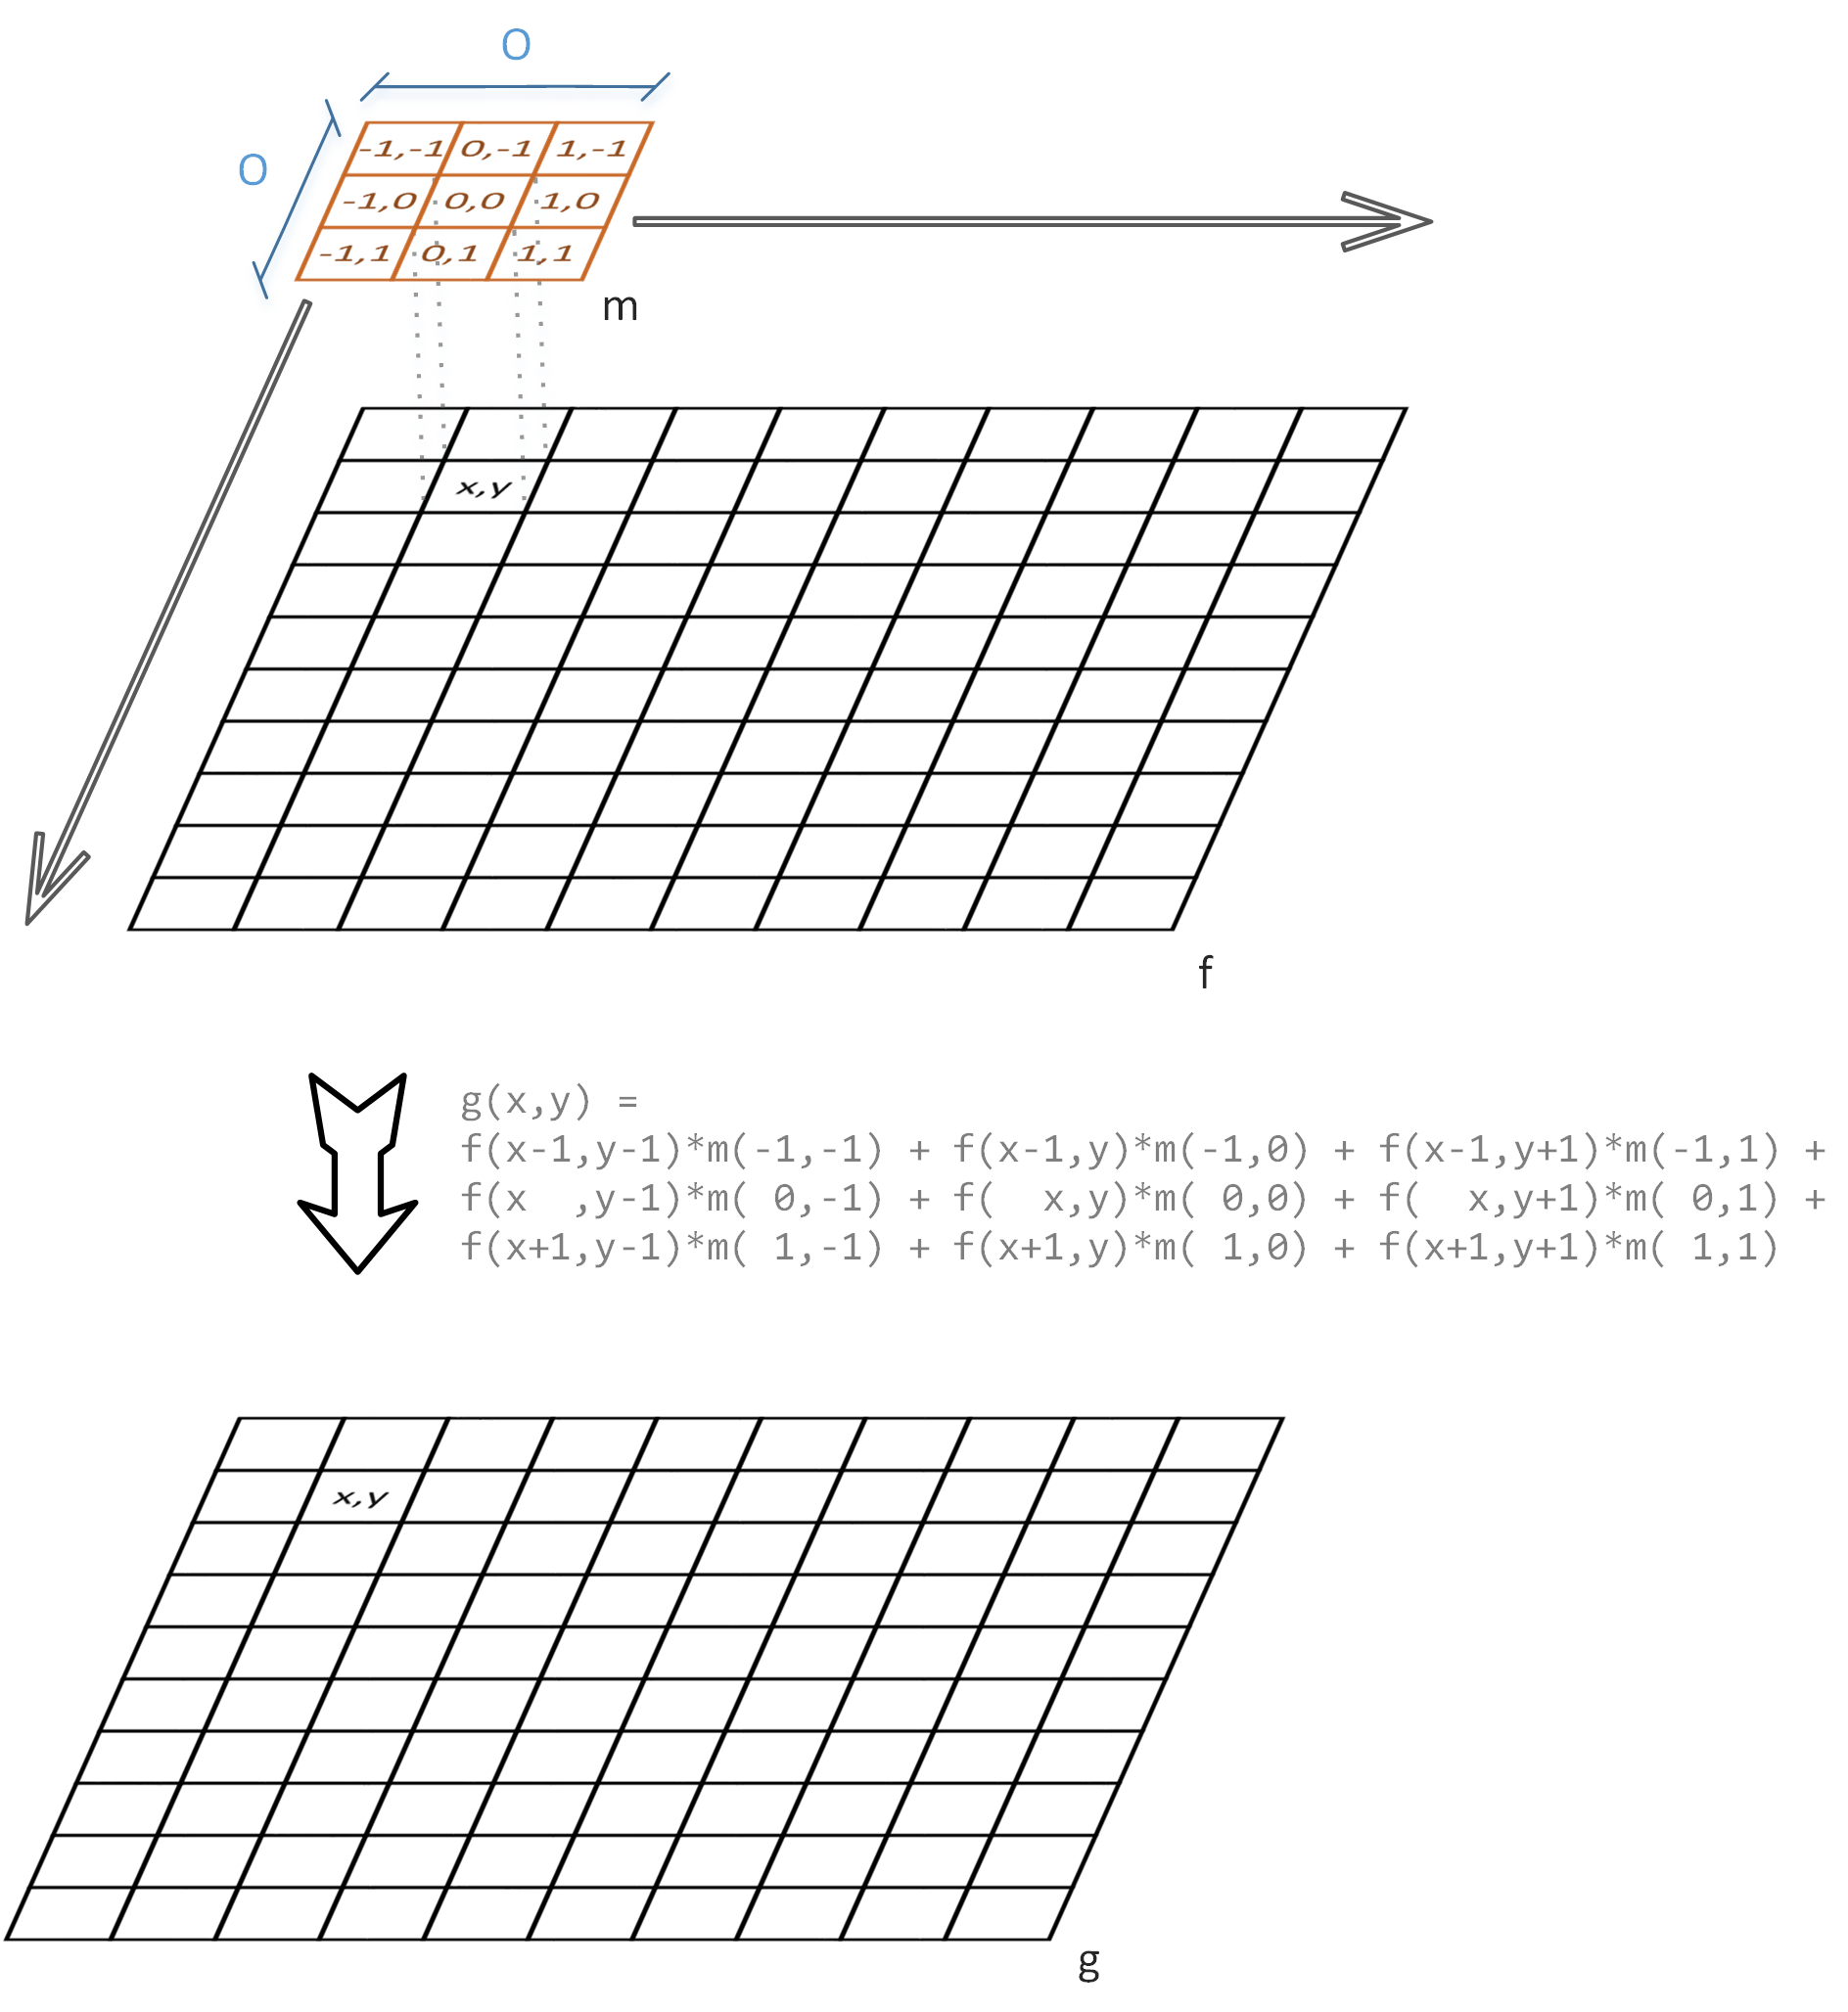
\includegraphics[scale=0.55]{Figuras/Convolutio.png}
	\caption{Filtragem por convolução}
	\label{fig:Convolution}
\end{figure}

Observe que o elemento central da máscara fica posicionado sobre o ponto \((x,y)\) da imagem, para que se possa calcular o ponto \((x,y)\) de \(g\) efetuando a convolução de \(f\) por \(m\). Observe ainda, que a matriz de convolução, para gerar toda a imagem \(g\), percorrendo todos os pontos de \(f\)  e aplicando a convolução ponto a ponto. E note também, no cálculo de \(g(x,y)\) na figura, que a convolução faz a soma das multiplicações entre os elementos da matriz \(m\) com a imagem \(f\), de modo que os índices dos elementos estejam sempre nas mesmas posições, ou seja, o ponto \((x,y)\) de \(f\) será multiplicado pelo elemento \((0,0)\) de \(m\), o ponto \((x+1,y)\) de \(f\) será multiplicado pelo elemento \((1,0)\) de \(m\), e assim por diante.

Com isso pode-se elaborar um algoritmo para processar uma imagem \(f\) sob uma matriz de convolução \(m\) dadas, ambas na forma de matriz de valores, de modo a se gerar uma imagem resultante \(g\) a partir da convolução da matriz \(m\) sobre a imagem \(f\), como mostrado a seguir no algoritmo \ref{alg:Convolution}:

\begin{algorithm}[H]
\SetAlgoLined
\KwData{
\\m \(\Rightarrow\) Matriz de convolução.
\\f \(\Rightarrow\) Imagem Inicial.
\\w \(\Rightarrow\) Largura da imagem em pixels.
\\h \(\Rightarrow\) Altura da imagem em pixels.
\\o \(\Rightarrow\) Ordem da matriz de convolução.

}
\KwResult{g - Imagem resultante da convolução de m sobre f }
Inicializar g como uma nova matriz[w][h] com zeros\;
\Para{$x \leftarrow $0 \KwTo $w$}
{
  \Para{$y \leftarrow $0 \KwTo $h$}
  {
    OffsetX - x - (int)(o/2)\;
    \Para{$i \leftarrow $0 \KwTo $o$}
    {
      OffsetY = y - (int)(o/2)\;
      \Para{$j \leftarrow $0 \KwTo $o$}
      {
        \Se{! (OffsetX < 0 OU\\ OffsetX >= w OU\\ OffsetY < 0 OU\\ OffsetY >= w) }
        {
        g[x][y] = g[x][y] + f[OffsetX][OffsetY] * m[i][j]\; 
        }
        OffsetY++\;
      }
      OffsetX++\;
    }
  }
}
\caption{Algoritmo de convolução de imagens}
\label{alg:Convolution}
\end{algorithm}

O algoritmo apresentado é o mais simples possível, e é otimizado para a rápida execução da tarefa, portanto ele não apresenta alguns recursos extras, que geralmente aparecem em algoritmos de convolução de imagens digitais, como a adição de um fator de multiplicação \(r\) e de um fator de soma \(baias\), que altera a imagem resultante g gerada, de modo que o fator \(r\), geralmente dentro do intervalo \([0,1]\), multiplica todos os elementos da imagem após o cálculo do ponto, e analogamente, o fator de soma \(baias\), que soma todos os elementos calculados da imagem resultante \(g\).  Tais fatores, no caso deste trabalho não são necessários, pois a matriz de convolução será gerada a partir de um algoritmo evolutivo, que já integra tais valores nos próprios elementos da matriz de convolução, caso seja necessário. Outro fato interessante a se analisar é que este algoritmo utiliza muito processamento e é diretamente dependente do tamanho da imagem e da máscara de convolução, pois, tomando como exemplo uma matriz de tamanho 5x5 e uma imagem 100x100, haverão 250000 multiplicações e 250000 somas para gerar a imagem final como resultado da convolução entre a imagem e a matriz.

Os filtros ou matrizes de convolução, quando aplicados sobre imagens, utilizando a técnica mostrada anteriormente tem diversas aplicações, como nas áreas de pré-processamento, remoção de ruídos, segmentação, suavização, detecção de bordas, etc.. No caso deste trabalho, é apresentado uma nova aplicação, dentro de uma metodologia que leva a geração de uma imagem resultante a qual representará uma imagem futura a partir de imagens anteriores.